\section{Use Case-Diagramm}

\begin{tcolorbox}
    Ein \textbf{Use Case-Diagramm} (\textbf{Anwendungsfalldiagramm}) zeigt Akteure und Anwendungsfälle und die Beziehungen zwischen diesen.
\end{tcolorbox}

\noindent
Ein \textbf{UML} \textbf{Use Case-Diagramm} besteht i.d.R. aus vier Elementen (s. Abbildung~\ref{fig:usecasediagram}):

\begin{enumerate}
    \item \textbf{Systeme} (Quadrate)
    \item \textbf{Anwendungsfälle} (Ellipsen)
    \item \textbf{Akteure} (Strichmännchen)
    \item \textbf{Assoziationen} (Verbindungslinien)
\end{enumerate}


\begin{figure}
    \centering
    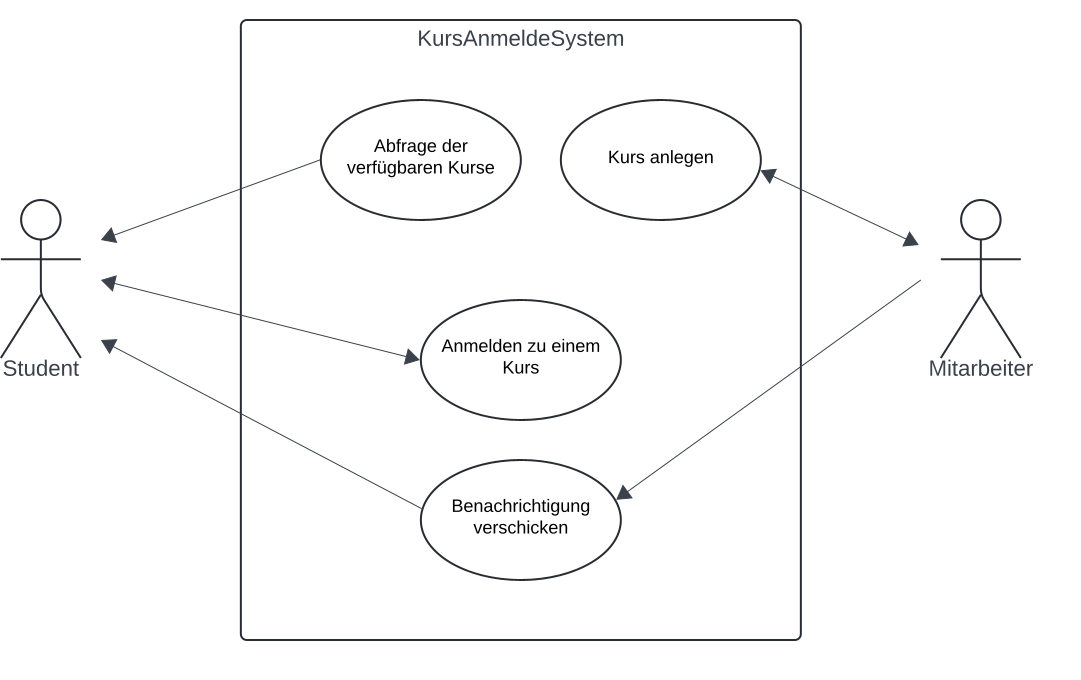
\includegraphics[scale=0.4]{chapters/Anhang/CheatSheets/img/usecasediagram}
    \caption{Beispiel eines Use Case-Diagramms. (Quelle: in Anlehnung an \cite[Figure A-1]{Mar03})}
    \label{fig:usecasediagram}
\end{figure}